\documentclass[11pt]{article}

\usepackage{layout}
\usepackage{lipsum}


\title{Test Dokument}
\author{Hofer}
\date{\today}

\begin{document}
\maketitle
BDA Test


\clearpage
\tableofcontents

\clearpage
\section{Abstract}

\lipsum

\clearpage
\section{Einleitung}


Ein \textbf{fettes} Brot.
\\Ein \textit{kursives} Brot.

Normales Brot\\
\textrm{Was ist rm}\\
\textsc{Was ist sc}\\
\textsf{Was ist sf}\\
\textsl{Was ist sl}\\
\texttt{Was ist tt}\\
\textup{Was ist up}\\


\clearpage
\section{Hauptteil}

% Verlinkungen
Siehe Kapitel \ref{sec:diskusion} \nameref{sec:diskusion}.\\
Hier mal ein Test Bild siehe \autoref{Fig:Kurfirsten}
% anstelle auto kann page stehen, oder nichts, dann ohne Abbildung. oder name.

%Buch zitieren, inhalt in {} steht im Tietze.bib zu oberst
Siehe Buch \cite{tietze1978advanced}

%Bild
\begin{figure}[h!] % h! ist es hier. t für Top. b für Bottom
\centering % so ist bild in der mitte
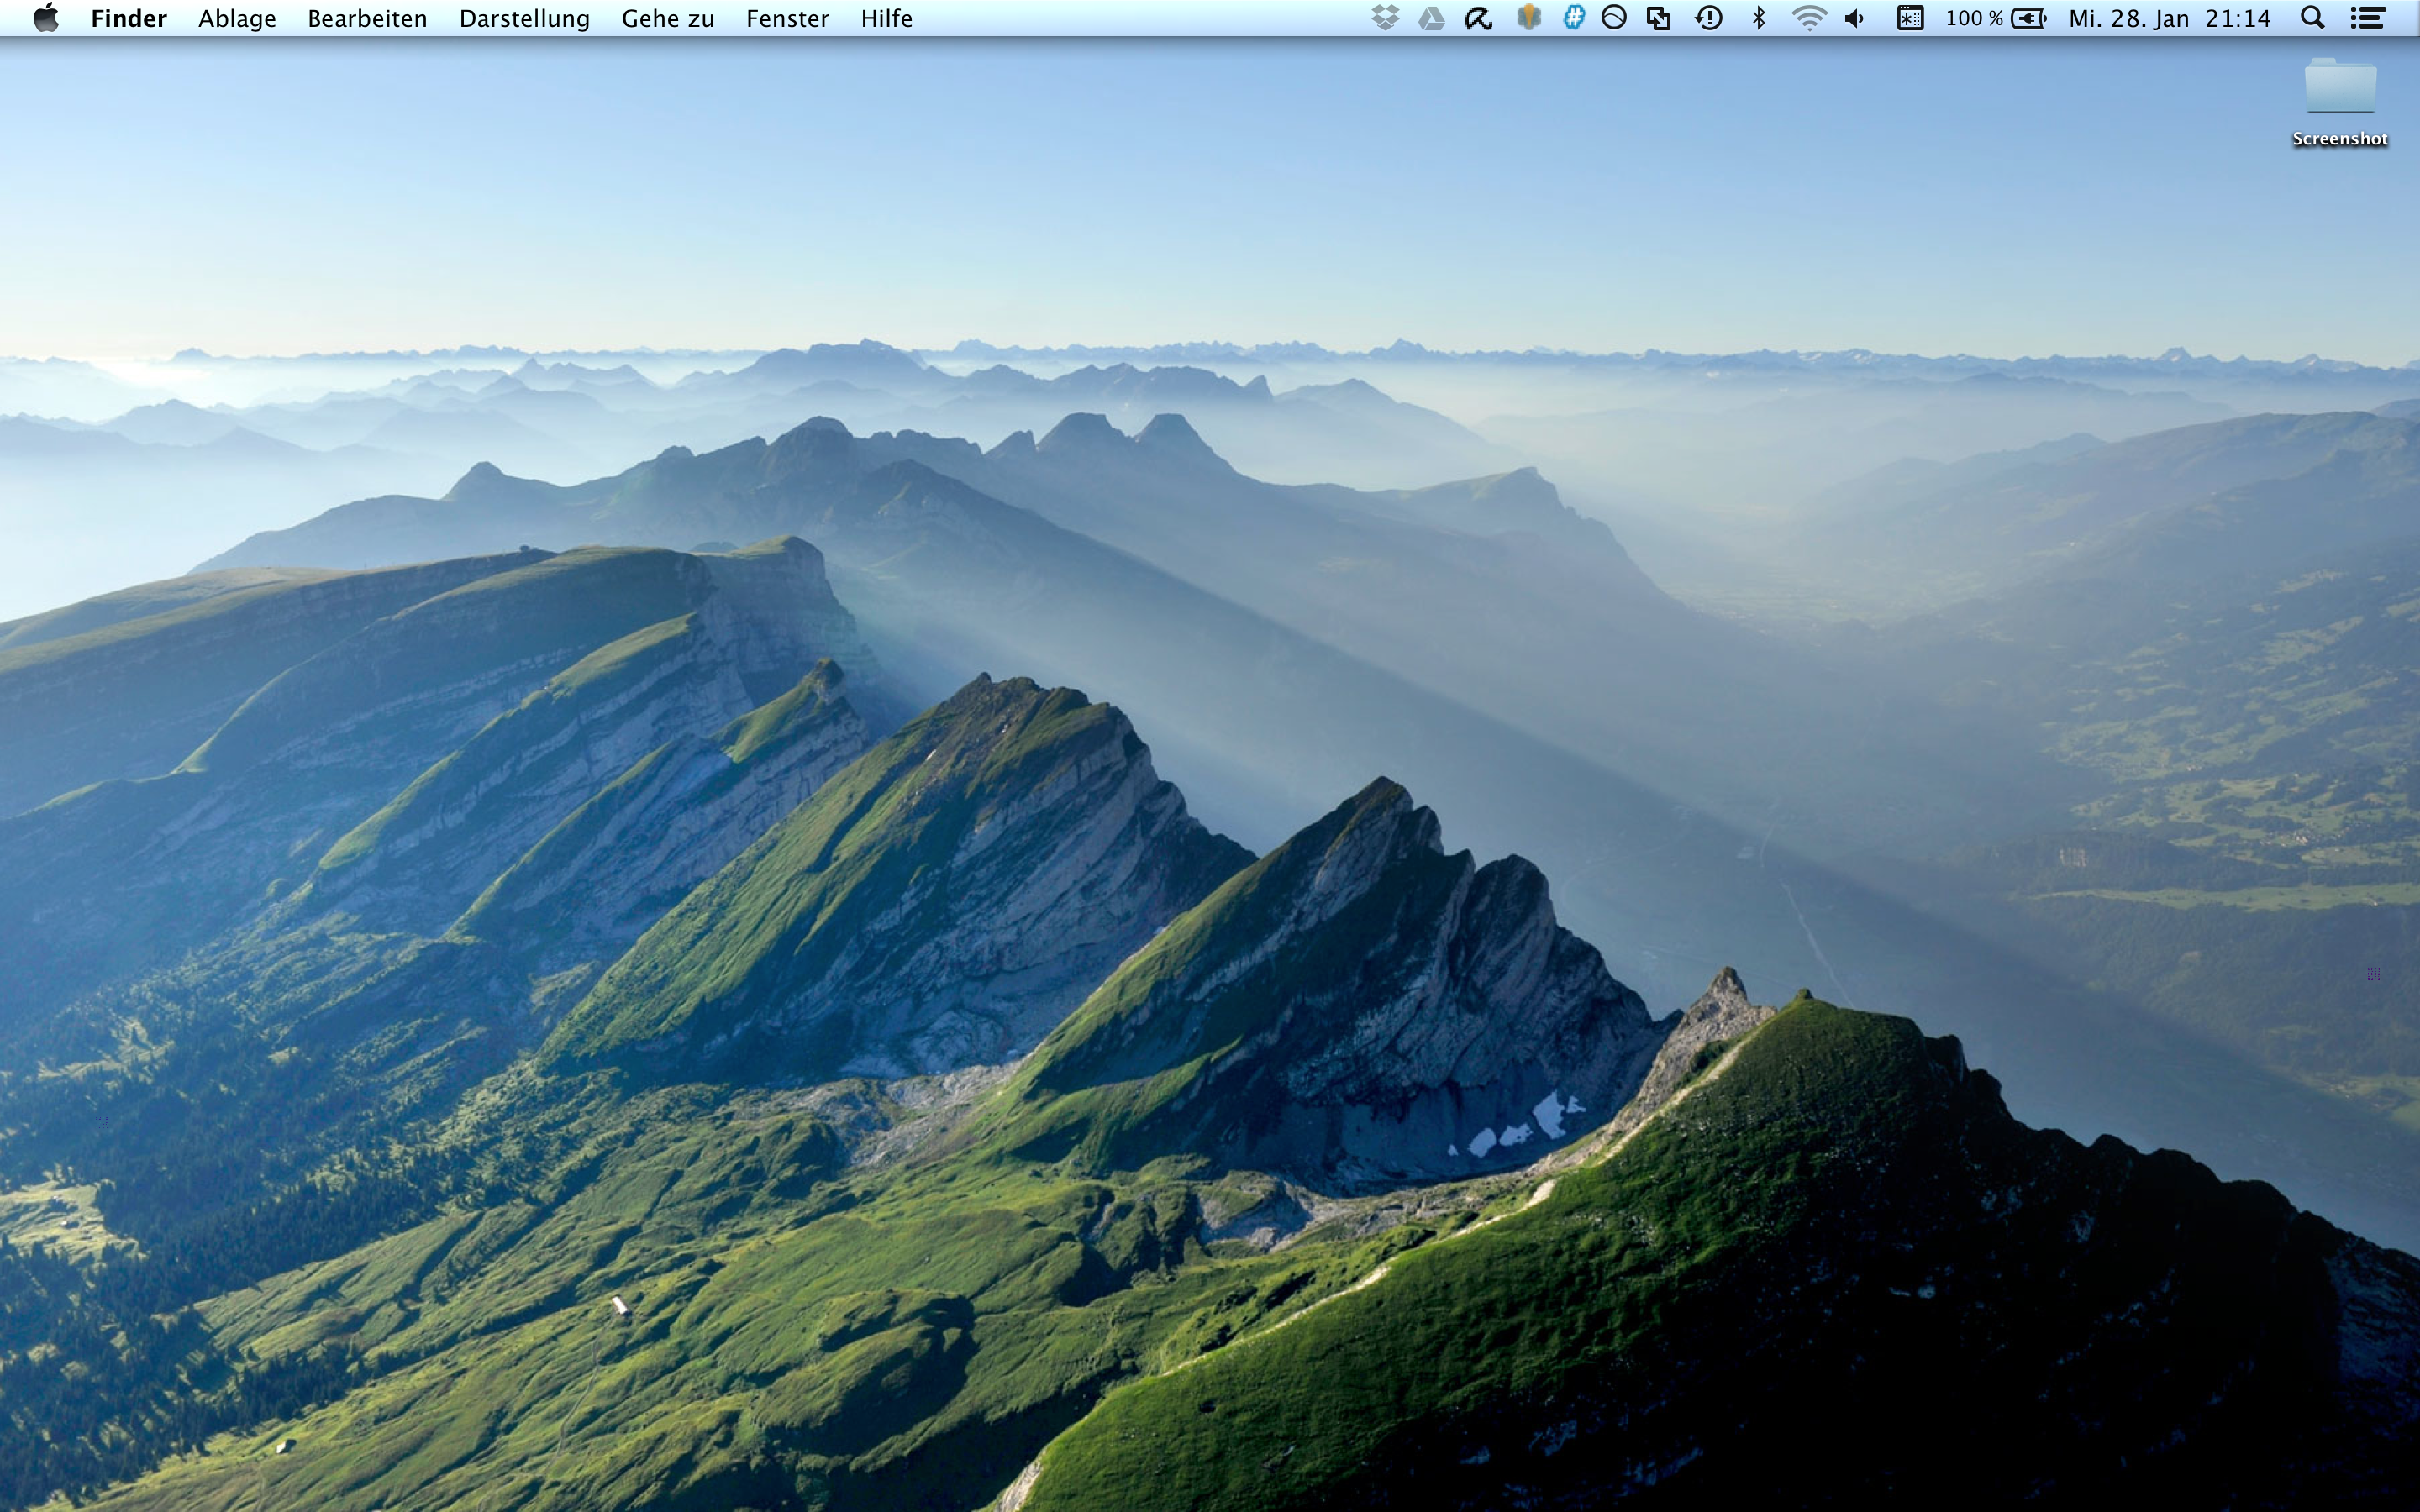
\includegraphics[width=0.7\textwidth]{Bilder/Kurfirsten.png}%width heisst 0.7 mal textbreite
\caption{Geili huärä Ussicht}
\label{Fig:Kurfirsten}
\end{figure}


\clearpage
\section{Diskussion}

\label{sec:diskusion}












\clearpage
% das \nocite{*} nimmt alles noch in Literatur was nicht zitiert wurde
\nocite{*}
\bibliography{Tietze.bib} % wenn mehrere dann mit komma trennen
\end{document}



